\title{%
  The terminal: Useful commands
}
\author{Daniel Bosk}
\institute{%
  KTH EECS
}

\mode<article>{\maketitle}
\mode<presentation>{%
  \begin{frame}
    \maketitle
  \end{frame}
}

\mode*


\begin{frame}
  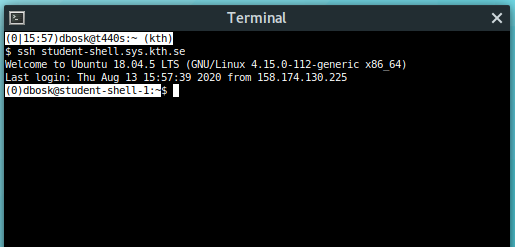
\includegraphics[width=\columnwidth]{../../ssh/terminal.png}
\end{frame}


\section{Manual pages}

\begin{frame}[fragile]
  \begin{center}
    \LARGE
    \lstinline[basicstyle=\LARGE]{man apropos}
  \end{center}
\end{frame}


\section{The file system}

\begin{frame}
  \begin{figure}
    % Define styles for dirs and files
    \tikzstyle{dir} = [text centered]
    \tikzstyle{file} = [rectangle, text centered]
    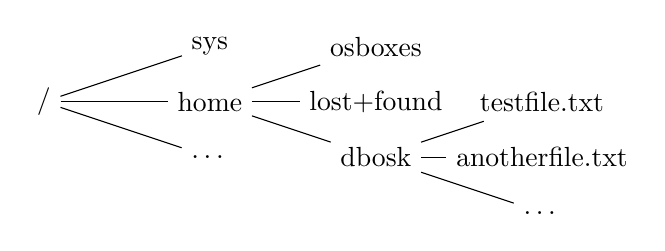
\begin{tikzpicture}[%
        grow=right, sloped, sibling distance=2em, level distance=6em
      ]
      \node[dir] {/}
        child {
          node[dir] {\dots}
        }
        child {
          node[dir] {home}
            child {
              node[dir] {dbosk}
                child {
                  node[file] {\dots}
                }
                child {
                  node[file] {anotherfile.txt}
                }
                child {
                  node[file] {testfile.txt}
                }
            }
            child {
              node[dir] {lost+found}
            }
            child {
              node[dir] {osboxes}
            }
        }
        child {
          node[dir] {sys}
        };
    \end{tikzpicture}
    \caption{The file system is a tree.}
  \end{figure}

  \begin{block}<2>{Navigating the file system}
    \begin{columns}[T]
      \begin{column}{0.5\columnwidth}
        \begin{itemize}
          \item \lstinline{pwd}
          \item \lstinline{cd}
          \item \lstinline{ls}
        \end{itemize}
      \end{column}
      \begin{column}{0.5\columnwidth}
        \begin{itemize}
          \item Special directories \lstinline{.} and \lstinline{..}
        \end{itemize}
      \end{column}
    \end{columns}
  \end{block}
\end{frame}

\begin{frame}[fragile]
  \begin{exercise}[What do the following commands do?]
    \begin{center}
      \lstinline[basicstyle=\Large]{mkdir rmdir touch cp mv rm}
    \end{center}
  \end{exercise}
\end{frame}

\begin{frame}[fragile]
  \begin{exercise}[What do the following commands do?]
    \begin{center}
      \lstinline[basicstyle=\Large]{cat less head tail grep file nano}
    \end{center}
  \end{exercise}
\end{frame}


\section{An exercise}

\begin{frame}[fragile]
  \begin{block}<+>{What we've learned}
    \begin{description}
      \item[Navigation] \lstinline{pwd cd ls .. .}
      \item[Files] \lstinline{mkdir rmdir touch cp mv rm}
      \item[Contents] \lstinline{cat less head tail grep file nano}
    \end{description}
  \end{block}

  \begin{exercise}
    \begin{itemize}
      \item Which commands must you run (and in which order) to get the same 
        output?
    \end{itemize}
    \begin{lstlisting}[numbers=none]
$ grep "contents" testfiles/testfile.txt
contents of testfile.txt
contents of testfile.txt
contents of testfile.txt
    \end{lstlisting}
  \end{exercise}
\end{frame}

\begin{frame}[fragile]
  \begin{solution}<+>[One alternative]
    \begin{lstlisting}[numbers=none]
mkdir testfiles
cp testfile.txt testfiles/
nano testfiles/testfile.txt
    \end{lstlisting}
  \end{solution}
  \begin{solution}<+>[Another alternative]
    \begin{lstlisting}[numbers=none]
mkdir testfiles
nano testfiles/testfile.txt
    \end{lstlisting}
  \end{solution}
\end{frame}


%%% REFERENCES %%%

%\begin{frame}[allowframebreaks]
%  \printbibliography{}
%\end{frame}
